\documentclass[a4j,12pt,onecolumn,oneside,notitlepage,openany,jarticle,final]{jreport}%両面刷り
%
\usepackage{cite}
\usepackage{makeidx,graphicx,epsbox,delarray}
\usepackage{fancyhdr,hhline,array}
\usepackage{pifont}
\usepackage{amssymb}
\usepackage{subfigure}
\usepackage{multirow}
\usepackage[dvipdfmx]{}
\usepackage{otf}
\usepackage{here}
\usepackage{url}
\renewcommand{\bibname}{参考文献}
\bibliographystyle{junsrt} 
%余白の設定 A4は縦297mm 横210mm 初期余白25.4mm
\topmargin=4.6mm %上余白 ヘッダをいれて30mmにする(4.6=30-25.4)その後微調整
\oddsidemargin=6.6mm %左余白 40mm=25.4+14.6
\textwidth=158mm %適当に決めました(155=210-40-15)
\textheight=252.5mm %同様に↑(232=297-40-25)
\makeindex
\date{}
%ページ番号を各ページ下に表示
\pagestyle{fancy}
% ヘッダの下線を引かない。
\lhead{}
\chead{}
\rhead{}
\renewcommand{\headrulewidth}{0.0pt}
\renewcommand{\footrulewidth}{0.0pt}
%以下「\UTF{2460}」等の囲い文字を使うための新しいコマンドを定義
\newcommand{\MARU}[1]{{\ooalign{\hfil#1\/\hfil\crcr
\raise.167ex\hbox{\mathhexbox20D}}}}
%
% 本文の行数と桁数を指定出来るように
\def\linesparpage#1{\baselineskip=\textheight
\divide\baselineskip by #1}
\def\kcharparline#1{%
\ifx\xkanjiskip\undefined%
% NTT jTeX用
\jintercharskip 0mm plus 0.2mm minus 0.2mm
\else
% ASCII pTex用
\xkanjiskip 0mm plus 0.2mm minus 0.2mm
\fi
\settowidth{\textwidth}{}%
\multiply\textwidth by #1}
%
%%% Document Start %%%%%%%%%
%
\begin{document}
%タイトルページ
\begin{titlepage}
\begin{center}
%
\vspace{20pt}
{\fontsize{50pt}{0pt}\selectfont \bf 関西大学 \\ \vspace{12pt} システム理工学部 \\ \vspace{12pt} 卒業論文} \\ %タイトル
\vspace{50pt}
%
{\fontsize{25pt}{0pt}\selectfont \underline{2022年度}} \\
\vspace{30pt}
{\fontsize{25pt}{0pt}\selectfont \bfseries
	\underline{対話型進化計算} \\
	\vspace{7pt}
	\underline{性格特性を表現} \\
	\vspace{7pt}
	\underline{ロボットジェスチャの最適化}
} \\
\vspace{30pt}
%
{\fontsize{22pt}{0pt}\selectfont 電気電子情報工学科} \\
\vspace{30pt}
{\fontsize{22pt}{0pt}\selectfont \underline{学籍番号 電19-0188} \\}
\vspace{15pt}
\underline{{\fontsize{22pt}{0pt}\selectfont 氏 名}\hspace{11pt}{\fontsize{30pt}{0pt}\selectfont 三河 亮斗}} \\
\vspace{15pt}
\underline{{\fontsize{22pt}{0pt}\selectfont 指導教授}{\fontsize{30pt}{0pt}\selectfont \hspace{5zw}}{\fontsize{12pt}{0pt}\selectfont 印}} \\
\vspace{25pt}
%
\fbox{{\fontsize{28pt}{0pt}\selectfont 感性情報システム研究室}} \\
\end{center}
\end{titlepage}
%フォントサイズと行間を指定
\fontsize{12pt}{21pt}
\selectfont
% 一ページを30行に
\linesparpage{30}
%タイトルと要旨はページ番号を出力しない
\pagestyle{empty}
%
\topmargin=-20.6mm %上余白 ヘッダをいれて30mmにする(4.6=30-25.4)その後微調整
\oddsidemargin=6.6mm %左余白 40mm=25.4+14.6
\textwidth=155mm %適当に決めました(155=210-40-15)
\textheight=252.5mm %同様に↑(232=297-40-25)
%目次のページ番号をローマ数字に指定
\addtolength{\textheight}{-12truemm}
\setcounter{page}{1}
\pagenumbering{roman}
\pagestyle{fancy}
%目次出力
\tableofcontents

\topmargin=-8.6mm %上余白 ヘッダをいれて30mmにする(4.6=30-25.4)その後微調整
\oddsidemargin=6.6mm %左余白 40mm=25.4+14.6
\textwidth=155mm %適当に決めました(155=210-40-15)
\textheight=240.5mm %同様に↑(232=297-40-25)

% !TEX root = MasterPaper.tex
\chapter{序論}
\thispagestyle{fancy}
\lhead{}
\chead{}
\rhead{}
\lfoot{} 
\cfoot{\thepage}  
\rfoot{}
%目次のページ番号をアラビア数字に指定
\setcounter{page}{1}
\pagenumbering{arabic}

近年世界で流行している新型コロナウイルス(COVID-19)の影響により,現地でのスポーツ観戦が困難になっている.
それに伴って,現地での観戦時特有の「臨場感」が失われてしまっていることが大きな問題となっている.

この問題を受け,近年ではKDDIと横浜DeNAベイスターズが実施するバーチャルハマスタなどの,次世代型のスポーツ観戦方式が登場している\cite{hamasuta}.
バーチャルハマスタとは,バーチャル空間にスタジアムを構築し,自宅からスマートフォンやパソコン,VRデバイスを使って観戦体験ができるプロジェクトである.
VR空間で,ユーザはオリジナルのアバターを用いて多くのファンと一緒に観戦し,コミュニケーションをとりながら球場の雰囲気を楽しむことができる.

しかし,この観戦方式は,観戦時にアバターが棒立ちになってしまうことや,感情表出方法が絵文字による表出のみであることから,現地でのスポーツ観戦を再現しきれておらず,臨場感を演出できていないと考えられる.
ここで,VR空間における棒立ちのアバターを感情表出を行うロボットに置き換えることで,現地でのスポーツ観戦を再現できる可能性がある.

一方で近年,自動運転を搭載した自動車が発表されるなど,人工知能を搭載した製品の普及は目覚ましいものとなっている.
使用者の暮らしに応じた機能を提示する人工知能搭載型の様々な電化製品が開発され,人工知能を搭載したロボットが囲碁でプロの棋士に勝利するなど,人工知能は人々にとって身近な存在になりつつある\cite{healsio}\cite{go}.

また,近年ではロボットに人工知能を搭載し,人とコミュニケーションをとるロボットが数多く登場している.
このようなロボットはコミュニケーションロボットと呼ばれており,その代表的なものにパーソナルロボットやペットロボットが挙げられる\cite{toyota}\cite{aibo}.
これらのロボットは人の心的状況を読み取り,感情的なコミュニケーションをとることが求められる.
さらに今後,公共の場で人の代わりにコミュニケーションをとるロボットが普及することが示唆されている\cite{deep}.

このようなコミュニケーションロボットは人と円滑なコミュニケーションを行うため,非言語情報による感情表現が重要だと言われている.
現在でも,顔表情で感情表出を行うロボットや,指と手によるジェスチャーとして手話を取り上げ,ロボットに実装した例が報告されている
\cite{kao}\cite{syuwa}.
コミュニケーションにおいて,人間に心的作用をもたらす要因は主として非言語情報である\cite{higengo}.
非言語コミュニケーションの重要性は,人間同士だけでなく,人間とロボットの場合においても同様であると考えられる.
したがって,人間と共存するコミュニケーションロボットには,非言語機能が必要になると考えられる.
そこで本研究では,非言語情報によって感情表出を行うロボット集団との試合観戦は,臨場感を演出できるか検証する.

本論文は5章で構成される.

第2章では,臨場感についての関連研究,スポーツ観戦における臨場感及び感性とロボットの関係性について述べる.
初めに,臨場感の定義と臨場感を感じる事象である「興奮」や「面白さ」の高まりに関する先行研究について述べる.
次に,スポーツ観戦における臨場感の演出に必要な要素について述べる.
最後に,ロボットに感性を導入する意義,ロボットと人間とのインタラクションについて述べる.

第3章では,スポーツ観戦における臨場感演出の定義,本研究で提案する内部モデルについての詳細及び実験環境,及び実験におけるロボット集団の動作について述べる.
本研究ではロボットが試合観戦中に感情表出をしているように見せる内部モデルを提案する.
また,本実験で用いたロボット集団とインタラクションをとる仮想環境と,仮想環境でのロボットの動作について述べる.

第4章では,提案ロボット集団との試合観戦が臨場感を演出できるか検証するための実験について述べる.
評価実験では,被験者は提案ロボット集団と比較ロボット集団の2集団と試合観戦を行い,アンケートによって試合観戦における臨場感,及びロボット集団への評価を行う.

第5章は結論であり,本研究により得られた成果についてまとめると共に,今後に残された課題について述べる.



% !TEX root = MasterPaper.tex
\chapter{関連研究}
\thispagestyle{fancy} % このページのみ
\lhead{}
\chead{}
\rhead{}
\lfoot{} 
\cfoot{\thepage}  
\rfoot{}
%

\section{臨場感}
\label{sec2.1}

\subsection{臨場感の定義}
\label{sec2.1.1}

「臨場感」とは,広辞苑第6版によると「現場にのぞんでいるような感じ」,大辞林初版によると「あたかもその場に臨んでいるような感じ」,大辞泉第2版によると「実際その場に身を置いているかのような感じ」のように,「あたかも」「その場に」「いるような」などの語を用いて定義されていることが多い\cite{rinjyo1}.

臨場感に関しては,多くの研究者がそれぞれの定義や概念を提唱している.定義や概念が数多く存在するため,臨場感という言葉の使われ方は,明らかに異なる視点のものを同じ言葉で呼んでいる場合も存在する.例えば Lombardらは,臨場感を社会的な相互作用,忠実な再現,移動,没入,メディアの中の人や物との社会的関係,メディアそのものとの社会的関係の6種類に分類している\cite{lombard}.一方で,安藤は,臨場感はいろいろな感覚の集合体であり,(1)立体感,質感,包囲感と呼ばれる空間的な要素,(2)ものの動感や同期している感覚といった時間的な要素,(3)自己存在感やインタラクティブ感,情感などを伴って自分自身がそこにいるように感じる身体的な要素,の3つの要素があるとしている\cite{ando}.

これらの研究より,臨場感というものは仮想的あるいは懐疑的な感覚体験であることを前提としている研究が多いことが分かる.しかしその一方で,日常的な言葉の表現としては,実際に存在する場面や対象に臨んでいる場合,まさにその体験をしている場合にも使用されることがあり,かなり広義の使用がなされている.




\subsection{臨場感に関する関連研究}
\label{sec2.1.2}
  
曖昧な「臨場感」の多義・多次元性の実態を明らかにするため,寺本らは,人間が臨場感を感じる事象の分析を行っている\cite{rinjyo2}.この研究によって,仮想的な感覚体験である「映画」や「映像」などの視聴覚メディアに関連した事象だけでなく,現実の目の前で行われているものである「ライブ・コンサート」や「スポーツ」などでも人間が臨場感を感じていることが明らかにされている.これらの事象は,興奮・緊張感・緊迫感などの「心を揺さぶる」「非日常体験」という点で共通する.したがって,人間が臨場感を感じる事象には,辞書で定義されている「その場にいるような感覚」とは別に,気持ちが昂るといった,「興奮」が必要であることが分かる.

また橋本らは,視聴覚メディアである「スポーツ観戦」において,興奮する場面,つまり臨場感を感じる場面について,観客の歓声量を用いた検証を行っている\cite{rinjyo3}.この研究では,野球観戦において,「得点が入るかもしれない」という場面では期待感が高まり,より興奮することが分かっている.したがって,観客は「面白さ」を高める場面で臨場感を感じていることが分かる.

このように,スポーツ観戦においても,仮想的な感覚体験とは別に,体験しているもの自体の面白さによって心が揺さぶられ,臨場感を感じていることが分かる.

\newpage

\section{スポーツ観戦における臨場感の演出}
\label{sec2.2}

先行研究において,臨場感を演出するためには,「その場にいるような感覚」と「興奮」の2つの要素が必要であると述べられている.
スポーツ観戦における臨場感は,「その場にいるような感覚」を集団が生み出す一体感と捉え,「興奮」は感情伝播を用いることで,2つの要素を満たすことができると考えられる.

そこで本節では,スポーツ観戦において臨場感の演出に必要な要素だと考えられる,集団が生み出す一体感と感情伝播について述べる.

\subsection{集団における一体感}
\label{sec2.2.1}

「一体」とは,ある個人と他者の「心的内容・心理状態」が一致,あるいは同じである状態を指す.そして「一体感」とは,「一体」を意識的,あるいは無意識的に感じている心的状態,心理を指す\cite{ittai}.一体感を得ることで,人々はよりその場にいるように感じることができるため,場面への没入感が増し,より大きな臨場感を得ることができると考えられる.スポーツ観戦においては,人々は自身と他者が同じチームを応援し,互いに感情表出を行うことで一体感を得ることができる.
    
\subsection{感情伝播}
\label{sec2.2.2}

「感情伝播」とは,他人の動作・表現・態度・発言を無意識に真似したり,同調したりすることで同じような気分になることである\cite{denpa}.例えば,周囲からポジティブな感情表現を刺激として受けた人は,ポジティブな感情を抱く傾向を持つ.また,感情伝播は物理的に近い人に起こりやすい傾向があると言われている.そのため,スポーツ観戦時の人が密集した空間では特に発生しやすいと考えられる.先行研究においても,スポーツ観戦を行う観客がプレーに反応して,強い感情伝播を起こすことが分かっている\cite{jyodo}.すなわち,感情伝播により,周囲の興奮から影響を受けることで興奮が高まり,より高い臨場感を得ることができると考えられる.

\newpage

\section{感性とロボット}
\label{sec2.3}

\subsection{ロボットの進化}
\label{sec2.3.1}

人間の代わりに過酷な作業を行う産業用ロボットは,1960年代に開発が進み,1980年代から工場の生産ラインなどに導入され,普及し始めた.この時代のロボットは作業場所も固定されており,単純な繰り返し作業をするというものだった.その後,ロボットの認識や記憶,学習などの能力向上により,様々な機能を持ったロボットが登場した.例えば,実際に利用されている警備ロボットや掃除ロボットは,作業場所が固定されておらず,屋内外を自由に動き回るような機能を有する.

現在では,産業用ロボットだけではなく,非産業用であるパーソナルロボットと呼ばれるロボットが登場している.パーソナルロボットとは,人間と密接に関わり合うことで,人間に快適な生活を積極的に提供してくれるロボットである\cite{perso}.例として,高齢者や障害者の手助けをする介護ロボットや,人間の心を和ませる動物の動きを模したペットロボット,人間とコミュニケーションをとるコミュニケーションロボットなどが存在している.




\subsection{ロボットへの感性導入}
\label{sec2.3.2}

近年開発されている家庭用ロボットや案内ロボットは,人と直接関わる機会が多いロボットである.これらのロボットが,人間の生活環境に適応するためには,人間同士のコミュニケーションを模倣した振る舞いを行う必要がある.例えば,人間同士のコミュニケーションでは,言語情報のみならず非言語情報のやり取りも重要な意味を持つ\cite{gengo}.非言語情報のうちでも特に,感情や情動などの心理的情報が重要である.また,ロボットは人間の感性表現を理解するだけでなく,感性を表現する機能も必要である.これらの感性に関する処理をロボットに導入することで,コミュニケーションによる親しみを生み出すことができる.このように,ロボットに感性を付け加えることで,ロボットの親しみやすさは増加すると言われている.

例えば,小林らは,ロボットが人の感情を認識し,それに対する反応を人にわかりやすいように表示伝達するためのアクティブ・ヒューマン・インターフェースを提唱し,この表示伝達方法として顔ロボットの顔表情による感性表現について調査を行っている\cite{gengo}.




\subsection{ロボット集団と人間のインタラクション}
\label{sec2.3.3}

近年では,ロボットが人間と同様に他者の反応を基に学習し,相互の繋がりを考慮した振る舞いをするロボットの研究などが行われている\cite{tekiou}.また,実際にパーソナルロボットも販売されており,人とロボットがコミュニケーションをとる機会は増えつつある\cite{rabot}.しかし,これらの想定するシチュエーションはあくまで1対1のコミュニケーションであり,ロボット集団と人間で行うコミュニケーションの実現には,達成すべき課題が数多く存在する.

ロボット集団と人とのインタラクションの実現には,人とロボットのコミュニケーションだけでなく,ロボット間でのコミュニケーションも必要である.ロボット間で行われる通信の多くは,赤外線などの人間には感知できない媒体を通して行われており,実際にコミュニケーションをとっているようには見えない.このような場合でも,ロボットが人間らしい振る舞いを行うことで,人はロボット同士がコミュニケーションを行っていると感じることができる.このように,ロボット集団とのインタラクションを行う人間は,ロボット同士がコミュニケーションを行う様子を観察することで,ロボット集団を対等なコミュニケーションの対象とみなすようになる.そして,ロボット集団と関係を築き,またロボット集団との自然なコミュニケーションを行うようになると考えられる.





\vspace{1cm}
\begin{figure}[!h]
 \begin{center}
  \centering
  \label{fig:kansei}
 \end{center}
\end{figure}



% !TEX root = MasterPaper.tex
\chapter{臨場感を演出する集団ロボットの内部モデル}
\thispagestyle{fancy} % このページのみ
\lhead{}
\chead{}
\rhead{}
\lfoot{} 
\cfoot{\thepage}  
\rfoot{}
%

\section{モデルの概要}
\label{sec3.1}

本研究では,ユーザは感情表出を行うロボット集団と共に野球観戦を行う.その中で,提案ロボット集団はユーザへの感情伝播を行い,観戦時特有の臨場感を演出することを目的とする.

本節では,野球観戦するロボットが試合状況を読み取って感情表出するための内部モデルを紹介する.初めに試合状況を読み取る方法について,次にロボットの表出する感情の生成方法について述べる.

\subsection{試合状況の読み取り}
\label{sec3.1.1}    

本研究では,ロボットは観戦する試合状況を読み取ることで,試合展開に沿った感情表出を行う.試合状況は,プロ野球情報サイトである「キューステ!」で利用されている「勝利確率グラフ」を用いて読み取る\cite{kyusute}.ここで,勝利確率グラフとは,特定の試合状況(イニング・点差・走者・アウトカウント)において,チームにどれだけ勝利が見込まれるかをグラフ化したものである.

勝利確率グラフで示される値である勝利確率$Q$は,過去のチームの勝利数$S$と過去の同じ状況の場面数$N$を用いて式(\ref{eq:3.1})のように算出する.勝利数$S$と場面数$N$の値は,1995年~2018年の日本プロ野球公式記録を参照する.2019年4月5日に開催された阪神タイガース-広島東洋カープの試合の勝利確率グラフの例を図\ref{win_percent}に示す.試合開始の時点では両チームにそれぞれ50%の勝利確率が見込まれ,回が進み点差が開くほど優位なチームは100%に近付いていく.また,得点期待の高いシーンや,終盤の勝敗に直結するシーンなどは勝利確率が大きく変動する.

\vspace{1cm}
 \begin{figure}[H]
 \begin{center}
  \centering
  \includegraphics[width=13.5cm]{images/chapter3/winper.eps}
  \caption{勝利確率グラフ}
  \label{win_percent}
 \end{center}
\end{figure}


\begin{equation}
\label{eq:3.1}
 Q = \frac{S}{N}
\end{equation}





\subsection{感情の生成方法}
\label{sec3.1.2}

先行研究では,野球観戦において得点に対する期待感が高まる場面で,観戦者の歓声量が増加することが分かっている\cite{rinjyo3}.つまり,観戦者は勝利の確率が変動する場面で,感情を表出しているといえる.そのため,ロボットが観戦者と同じような場面で感情表出を行うことで,ユーザはロボットと違和感なく野球観戦をすることができると考えられる.

そこで,本研究では,ロボットは勝利確率グラフの増減値の幅$W$を用いて感情の生成を行う.増減値の幅$W$は現在の勝利確率$Q_{a}$と1つ前の勝利確率$Q_{b}$を用いて式(\ref{eq:3.2})のように定義する.
\begin{equation}
\label{eq:3.2}
 W = \frac{Q_{a}-Q_{b}}{100}
\end{equation}

現在のシーンの勝利確率を$Q_{a}$,1つ前のシーンの勝利確率を$Q_{b}$とし,100で割ることによって勝利確率の増減値の幅を算出する.

提案するロボットは,喜の感情と哀の感情の2種類の感情を生成する.$W$の符号によって感情の種類を決定し,$W > 0$なら喜の感情を,$W < 0$なら哀の感情を表出する.


\newpage

\section{実験環境}
\label{sec3.2}

実環境でのインタラクションにおいて,感情を表出するロボット集団を準備することや,リアルタイムでの勝利確率を取得することは困難であるため,本実験では仮想環境であるVR空間を用いて実験を行う.本研究では,採用しているバーチャルアバターをロボットと呼ぶ.ロボット集団と共に野球観戦を行うため,スポーツバーを模した空間をゲームエンジンであるUnityを用いて制作している\cite{unity}.

本実験では,観戦を行う場所としてスポーツバーを模した内装と,感情を表出するロボット集団を,Unity内のAsset storeにある有償のAssetを改変して使用している\cite{bar}\cite{lilrobot}.スポーツバーとロボット集団の外観を図\ref{sports_bar},図\ref{robot}に示す.

また,Unityで作成したVR空間を体験するためのデバイスとして,ヘッドマウントディスプレイ,ヘッドフォンを使用する.この機器は家庭用VRデバイスであるHTC VIVEを用いる\cite{vive}.

本実験で使用するヘッドフォン付きヘッドマウントディスプレイを図\ref{Vive}に示す.


\vspace{1cm}
 \begin{figure}[H]
 \begin{center}
  \centering
  \includegraphics[width=15cm]{images/chapter3/sports_bar.eps}
  \caption{実験環境}
  \label{sports_bar}
 \end{center}
\end{figure}


\newpage

\vspace{1cm}
 \begin{figure}[!h]
 \begin{center}
  \centering
  \includegraphics[width=15cm]{images/chapter3/robot.eps}
  \caption{ロボット集団}
  \label{robot}
 \end{center}
\end{figure}


\vspace{1cm}
 \begin{figure}[!h]
 \begin{center}
  \centering
  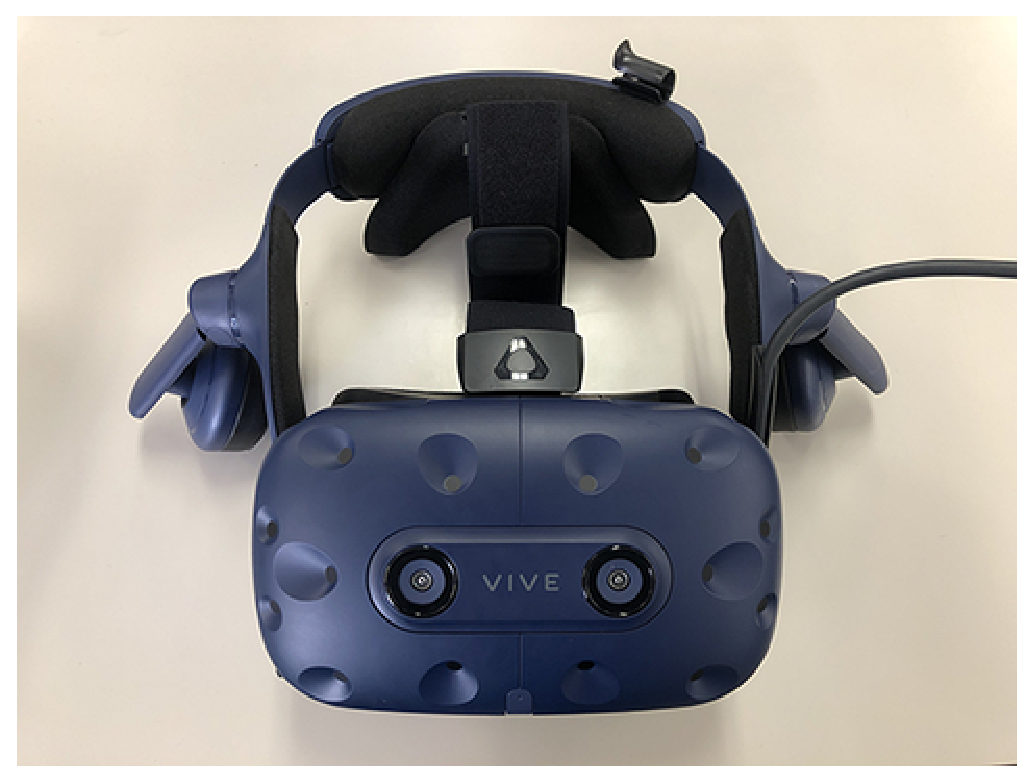
\includegraphics[width=12cm]{images/chapter3/Vive.eps}
  \caption{ヘッドマウントディスプレイ}
  \label{Vive}
 \end{center}
\end{figure}


\subsection{スポーツバーでの観戦}
\label{sec3.2.1}

実験中の画面の様子を図\ref{bar_scene}に示す.本実験では被験者とロボットのみで試合観戦を行う.共に試合観戦を行うロボット集団は,スポーツバーを模した空間上の席に着席して試合観戦を行う.

被験者はヘッドフォン付きヘッドマウントディスプレイを装着して着席し,その場から動かずにロボット集団と試合観戦を行う.図\ref{sports_bar}の前方にある4台のモニターに映し出される試合を観戦する.また,ヘッドマウントディスプレイによる映像だけでなく,ヘッドフォンからは観戦映像の音が流れている.このように,被験者は視覚情報と聴覚情報の2つを用いて試合観戦を行う.




\vspace{1cm}
 \begin{figure}[!h]
 \begin{center}
  \centering
  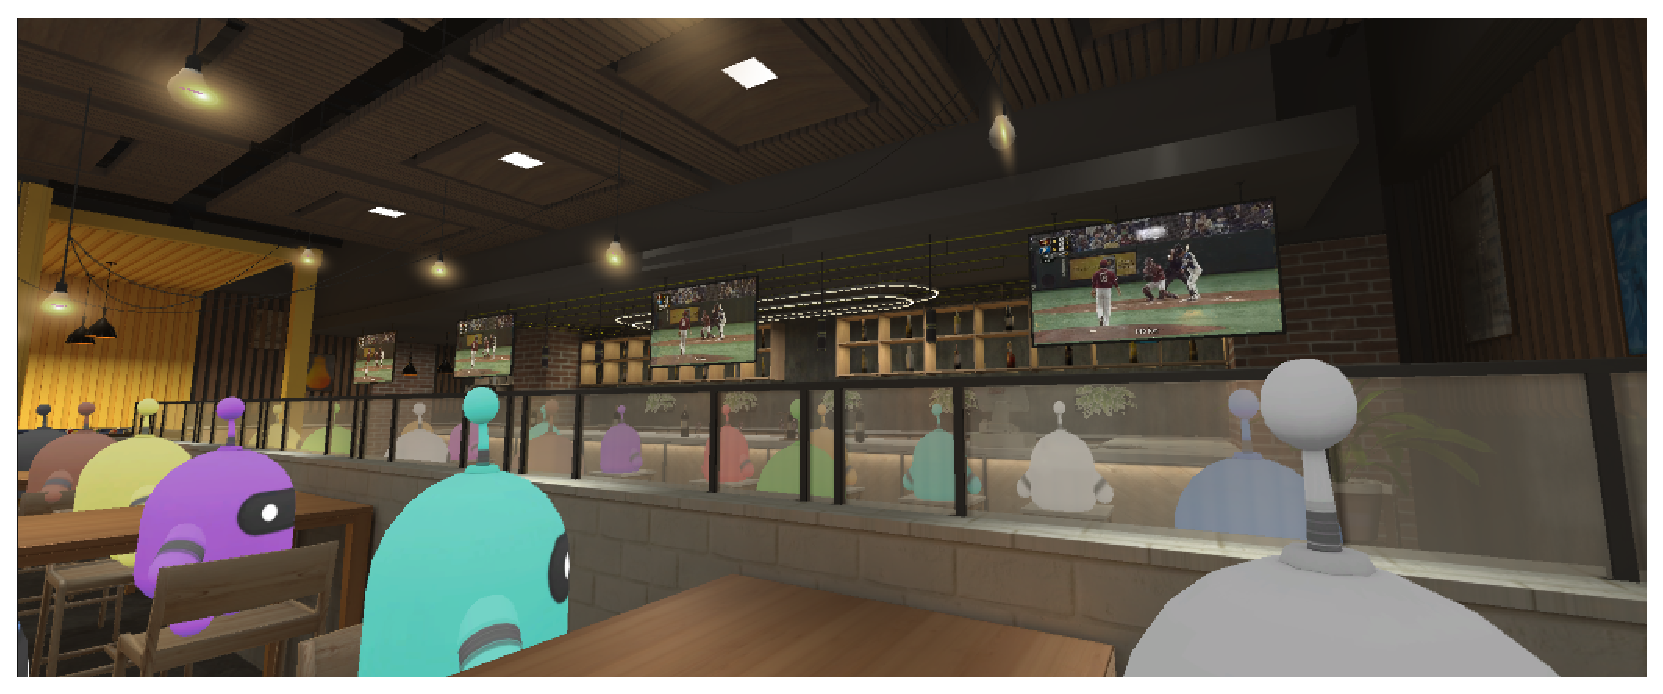
\includegraphics[width=15cm]{images/chapter3/bar_scene.eps}
  \caption{スポーツバーの様子}
  \label{bar_scene}
 \end{center}
\end{figure}



\newpage



\subsection{ロボット集団の動作}
\label{sec3.2.2}

被験者と共に試合観戦をするロボット集団は,感情表出しない状態(Idle状態),喜の感情表出,哀の感情表出を行う.

Idle状態では,ロボットは図\ref{Idle}の状態から,一定の周期でゆっくりと上下に反復運動を行う.この動作によって,人間の呼吸運動を再現する.また,各ロボットは,反復運動の速さを24回/分,27回/分,30回/分,33回/分,36回/分の5種類からランダムで設定されており,速さを変えることによってロボットの個性を設計している.

喜の感情表出は,図\ref{happy}のように,手を挙げながらジャンプする動作を繰り返すことで表出する.表出する感情の程度は,ジャンプする動作の速さを変更することで設計する.本実験では感情の程度を小,中,大の3種類に設定し,小なら30回/分,中なら50回/分,大なら70回/分の速さで感情表出を行う.

哀の感情表出は,図\ref{sad}のように,飛び上がって倒れこむ動作を繰り返すことで表出する.表出する感情の程度は,倒れこむ速さを変更することで設計する.喜の感情と同じく3段階の感情の程度を設定し,小なら12回/分,中なら15回/分,大なら20回/分の速さで感情表出を行う.


\vspace{1cm}
 \begin{figure}[!h]
 \begin{center}
  \centering
  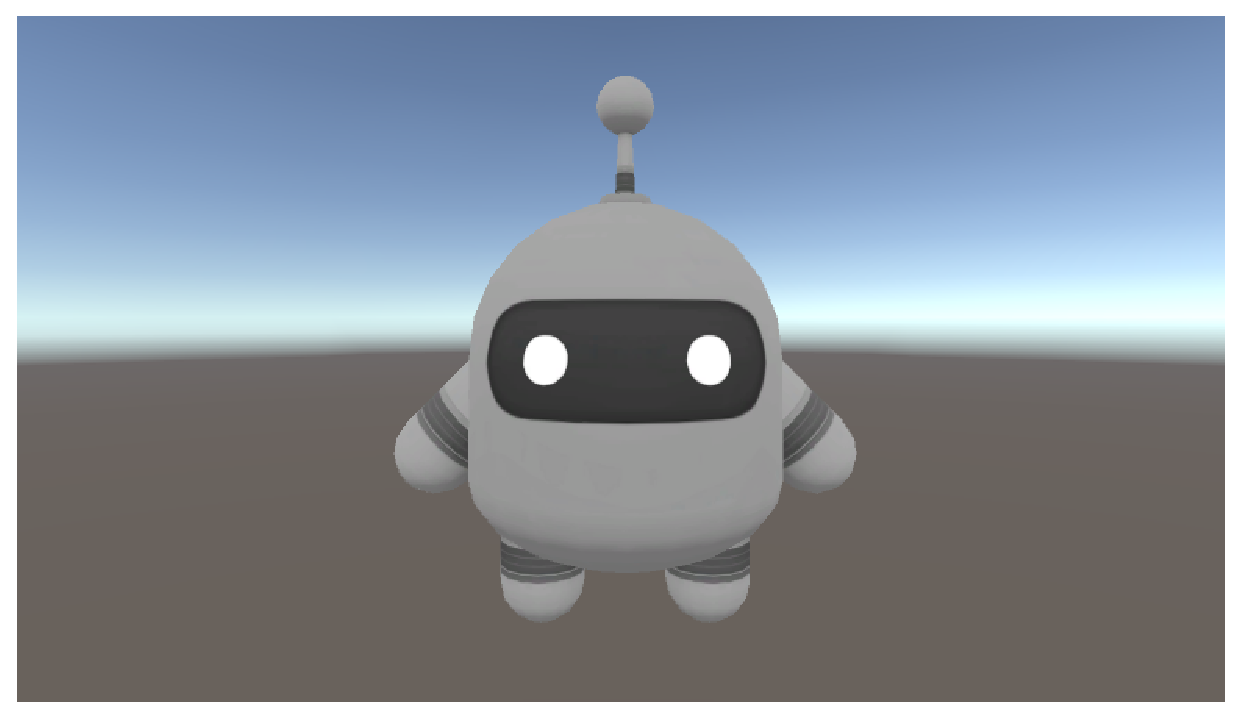
\includegraphics[width=12cm]{images/chapter3/Idle.eps}
  \caption{Idle状態のロボット}
  \label{Idle}
 \end{center}
\end{figure}

\vspace{1cm}
 \begin{figure}[!h]
 \begin{center}
  \centering
  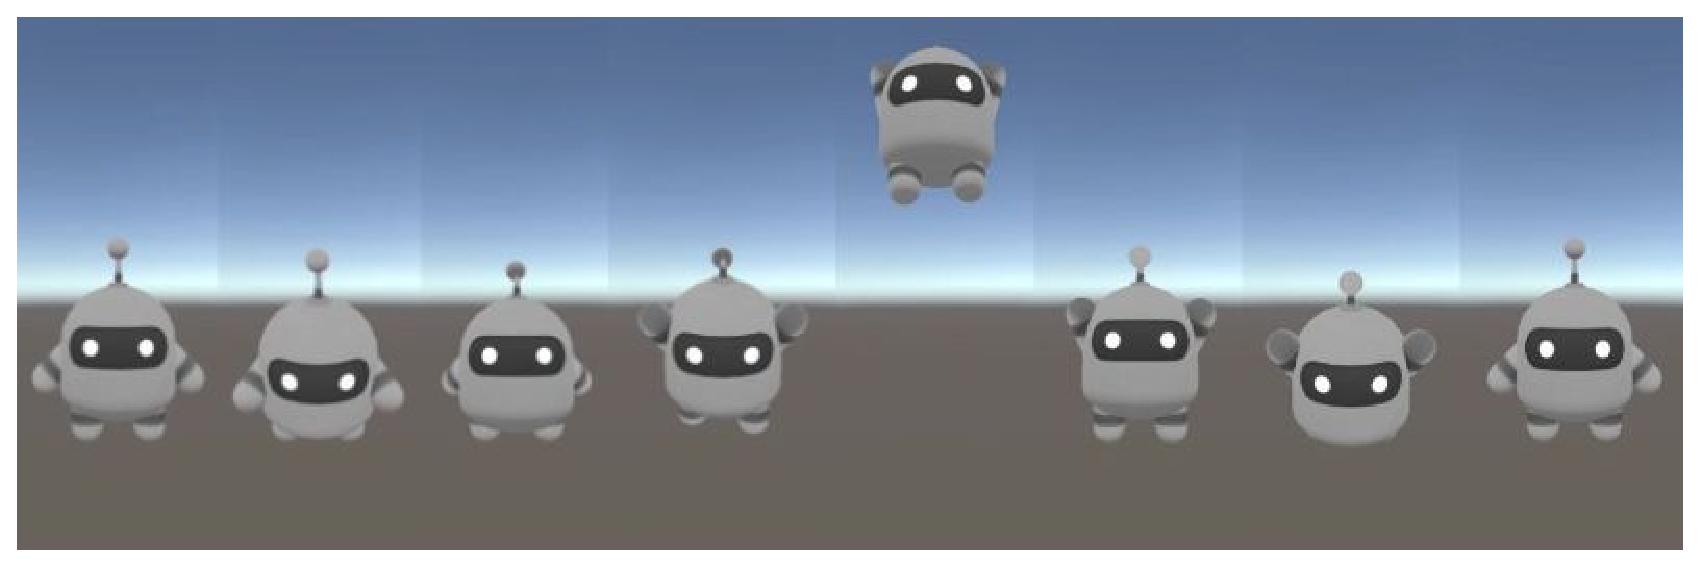
\includegraphics[width=12cm]{images/chapter3/happy.eps}
  \caption{喜の表出感情}
  \label{happy}
 \end{center}
\end{figure}

\vspace{1cm}
 \begin{figure}[!h]
 \begin{center}
  \centering
  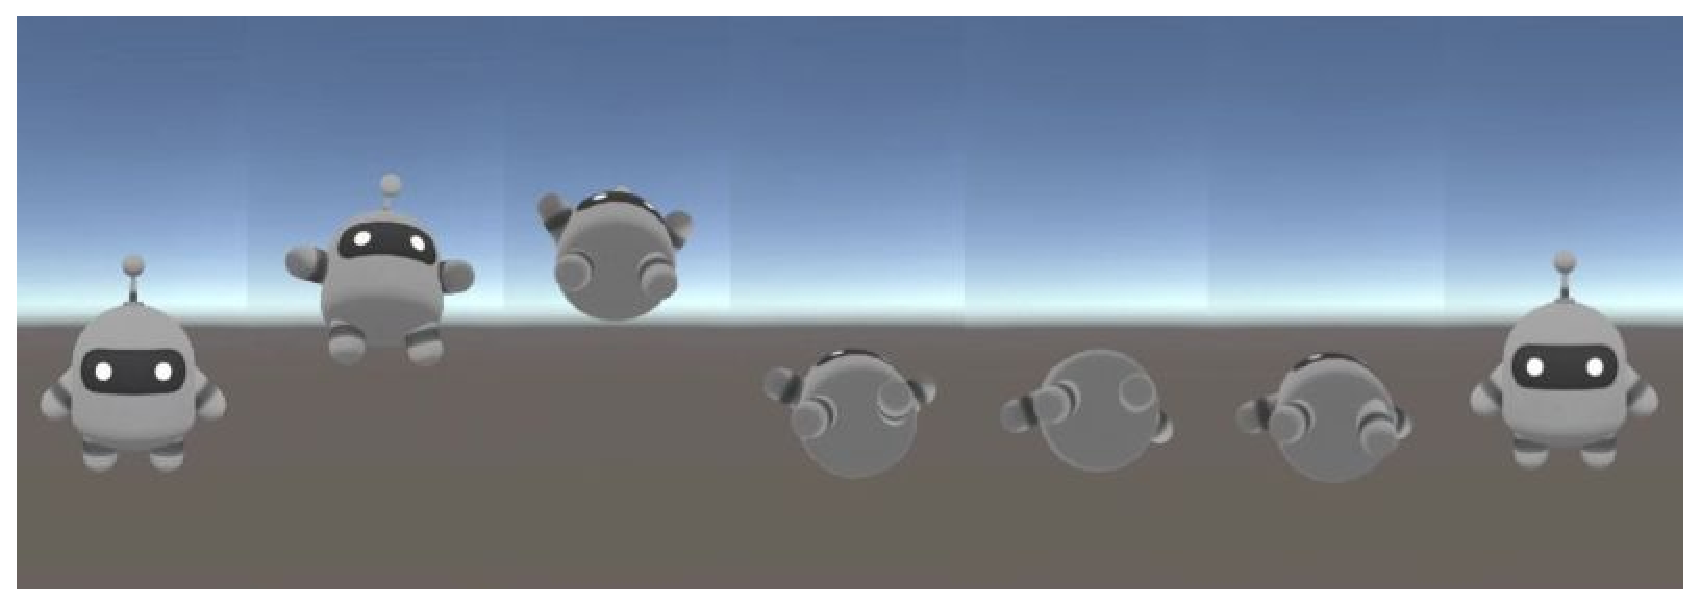
\includegraphics[width=12cm]{images/chapter3/sad.eps}
  \caption{哀の表出感情}
  \label{sad}
 \end{center}
\end{figure}

\newpage




















% !TEX root = MasterPaper.tex
\chapter{実ユーザによる評価実験}
\thispagestyle{fancy}
\lhead{}
\chead{}
\rhead{}
\lfoot{} 
\cfoot{\thepage}  
\rfoot{}
%

\section{実験概要}
\label{sec4.1}

本実験では,被験者にはヘッドマウントディスプレイを装着し,VR空間内のスポーツバーを模した空間で提案ロボット集団,比較ロボット集団と野球観戦を行ってもらう.比較ロボット集団とは感情表出の程度が異なるロボット集団である.感情表出の詳細については4.2.2で述べる.実験前に,被験者に対して本研究で示すスポーツ観戦における臨場感演出の定義について説明する.順序効果を防ぐため,被験者を提案ロボット集団,比較ロボット集団の順に観戦を行うグループと,比較ロボット集団,提案ロボット集団の順に観戦を行うグループに分ける.ロボット集団の総数は34体であり,被験者と同じチームを応援するロボットが22体,被験者と異なるチームを応援するロボットが12体になっている.ロボット集団の印象に関するアンケートは各ロボット集団との観戦後に回答してもらう.また,各ロボット集団の比較に関するアンケートは実験終了後に回答してもらう.

本実験の被験者は野球観戦に興味がある,また野球に関する知識がある20代の男女12名である.

ロボット集団の印象に関するアンケート項目を表\ref{question1}に示す.表\ref{question1}の計8つの質問に加えて自由記述からなるアンケートである.本アンケートはそれぞれ「そう思う/少しそう思う/どちらでもない/あまりそう思わない/そう思わない」の5段階で評価する.

Q1は,ロボット集団の感情表出によって観戦の楽しさに差が生まれるかを調査するための質問である.Q2~Q5は,ロボット集団との観戦で臨場感を演出することができるかを問う質問である.Q6~Q8はロボット集団への親和性を問う質問である.

次に,ロボット集団の比較に関するアンケート項目を表\ref{question2}に示す.表\ref{question2}の計7つの質問に加えて自由記述からなるアンケートである.本アンケートはそれぞれ「1回目のロボット集団/どちらかといえば1回目のロボット集団/どちらともいえない/どちらかといえば2回目のロボット集団/2回目のロボット集団」の5段階で評価する.

Q9は,ロボット集団の感情表出によって観戦の楽しさにどのくらいの差が生まれるかを調査するための質問である.Q10~Q12は,ロボット集団との観戦における臨場感演出の差を調査する質問である.Q13~Q15は,ロボット集団の親和性の差を調査する質問である.


\begin{table}[!ht]
\caption{ロボット集団の印象に関するアンケート項目}
\label{question1}
\begin{center}
\begin{tabular}{|l||l|}\hline
Q1&ロボット集団との観戦を楽しむことができたか\\ \hline
Q2&実際にロボット集団は観戦しているように感じたか\\ \hline
Q3&ロボット集団との観戦で一体感を感じることができたか\\ \hline
Q4&ロボット集団との観戦で臨場感を感じることができたか\\ \hline
Q5&ロボット集団の感情表出に感化されたか\\ \hline
Q6&ロボット集団に人間らしさを感じたか\\ \hline
Q7&ロボット集団に親しみを持てたか\\ \hline
Q8&またこのロボット集団と一緒に観戦したいか\\ \hline

\end{tabular}
\end{center}
\end{table} 

\begin{table}[!ht]
\caption{ロボット集団の比較に関するアンケート項目}
\label{question2}
\begin{center}
\begin{tabular}{|l||l|}\hline
Q9&どちらのロボット集団との観戦が楽しかったか\\ \hline
Q10&どちらのロボット集団に一体感を感じたか\\ \hline
Q11&どちらのロボット集団に臨場感を感じたか\\ \hline
Q12&どちらのロボット集団の感情表出に感化されたか\\ \hline
Q13&どちらのロボット集団に人間らしさを感じたか\\ \hline
Q14&どちらのロボット集団に親しみを持てたか\\ \hline
Q15&どちらのロボット集団とまた一緒に観戦したいか\\ \hline

\end{tabular}
\end{center}
\end{table} 

\clearpage

\section{実験条件}
\label{sec4.2}

\subsection{観戦する試合映像}
\label{sec4.2.1}

本実験では,被験者の疲労を考慮して,野球中継を8分程度にまとめたハイライト形式の映像を被験者に観戦してもらう.ハイライトは,日本プロ野球のパシフィック・リーグの試合を動画配信するインターネットテレビサービスである「パ・リーグTV」で提供されているアーカイブ動画を使用する\cite{patv}.
このアーカイブ動画を8分程度にまとめるため,試合内で勝利確率の増減値の幅$W$が$|W|\geq0.05$のシーンを切り抜き,繋げることで作成する.

本実験では,2021年4月16日に開催された北海道日本ハムファイターズ-東北楽天ゴールデンイーグルスの第4回戦と,同年4月18日に開催された同チームの第6回戦を用いて実験を行う.どちらも1-4で東北楽天ゴールデンイーグルスが勝利しており,試合展開は似通ったものになっている.2試合の勝利確率グラフを図\ref{0416},図\ref{0418}に示す.また,被験者には勝利チームを応援してもらう.




\subsection{ロボット集団のパラメータ}
\label{sec4.2.2}

提案ロボットと比較ロボットは感情表出のしやすさが異なる.

ロボットの感情表出の条件は以下のようになっており,式(\ref{eq:4.1})なら小の感情を,式(\ref{eq:4.2})なら中の感情を,式(\ref{eq:4.3})なら大の感情を表出する.
\begin{equation}
\label{eq:4.1}
 x \leq |W| \leq x + a
\end{equation}
\begin{equation}
\label{eq:4.2}
 x + a \leq |W| \leq x + 2a
\end{equation}
\begin{equation}
\label{eq:4.3}
 x + 2a \leq |W| 
\end{equation}


$W$は勝利確率の増減値の幅であり,$x$は各ロボットの感情表出のしやすさを表すパラメータである.また,$a$は感情の程度のパラメータである.$a$はハイライトに用いたシーンの増減値の平均値より決定しており,本実験では$a = 0.05$としている.

提案ロボットは,感情表出しやすいロボットである.提案ロボットが持つ,感情表出のしやすさを表すパラメータ$x$は,
$0.01 \leq x \leq 0.05$の範囲でランダムに与えられる.作成したハイライトは$|W| \geq 0.05$のシーンから構成されているため,全てのシーンで,少なくとも小の感情を表出する.

比較ロボットは提案ロボットとは異なり,勝敗が決定するシーン以外では感情表出せず,試合観戦を行うロボットである.比較ロボットのパラメータ$x$は,$0.15 \leq x \leq 0.20$の範囲でランダムに与えられる.このパラメータにより,比較ロボットはほとんどのシーンで感情表出を行わない.

\newpage

\vspace{1cm}
\begin{figure}[!h]
 \begin{center}
  \centering
  \includegraphics[width=13cm]{images/chapter4/0416.eps}
  \caption{2021年4月16日に行われた試合の勝利確率グラフ}
  \label{0416}
 \end{center}
\end{figure}


\vspace{1cm}
\begin{figure}[!h]
 \begin{center}
  \centering
  \includegraphics[width=13cm]{images/chapter4/0418.eps}
  \caption{2021年4月18日に行われた試合の勝利確率グラフ}
  \label{0418}
 \end{center}
\end{figure}


\newpage


\section{実験結果}
\label{sec4.3}

実験後に行うアンケート結果より,提案ロボット集団が被験者に臨場感を与えられたかを検証する.提案ロボット集団と比較ロボット集団への印象に関するアンケート結果を図\ref{Q1}~図\ref{Q8}に示す.また,実験終了後に行ったアンケート結果より,提案ロボット集団と比較ロボット集団を比較して,どのくらい臨場感の演出に差があったかを検証する.提案ロボット集団と比較ロボット集団の比較に関するアンケート結果を図\ref{Q9}~図\ref{Q15}に示す.

まず,ロボット集団の印象について問う質問であるQ1~Q8について述べる.Q1のアンケート結果より,被験者は頻繁に感情を表出する提案ロボット集団との観戦により,観戦時に楽しさが生じたことが分かる.Q2,Q3のアンケート結果より,提案ロボット集団との観戦で,被験者はロボット集団と共に観戦し,一体感を感じていたことが分かる.Q4のアンケート結果では,半数の被験者が提案ロボット集団への質問で「そう思う」「少しそう思う」と回答した.比較ロボット集団への質問では,被験者の大半が「あまりそう思わない」「そう思わない」と回答したことから,概ね臨場感が演出できていたと言える.Q5のアンケート結果より,被験者は提案ロボット集団の動作による感情表出に感化されたことが分かる.Q6,Q7,Q8のアンケート結果より,提案ロボット集団に親和性を感じていたことが分かる.


次に,ロボット集団の比較について問う質問であるQ9~Q15について述べる.Q9のアンケート結果より,91.7%の被験者が提案ロボット集団との観戦の方がより楽しかったと回答した.Q10のアンケート結果より,被験者全員が提案ロボット集団との観戦でより一体感を感じたと回答した.Q11のアンケート結果より,被験者全員が提案ロボット集団との観戦でより臨場感を感じたと回答した.Q12のアンケート結果より,91.7%の被験者が提案ロボット集団の方がより感化されたと回答した.Q13,Q14,Q15のアンケート結果より,提案ロボット集団の方が,より親和性を感じていることが分かる.

アンケートの自由記述欄には,提案ロボット集団について,「実際に人と一緒に観戦しているみたいで楽しかった」「動作だけでも一体となって楽しんでいる感覚があった」という,本実験の目的に沿った記述が多く見られた.また,比較ロボット集団について,「自分が喜んでいる時にロボットが喜んでおらず臨場感を感じることができなかった」といった記述が見られた.こちらも,本実験の目的に沿っていると言える.一方で,ロボット集団の感情表出方法として,歓声による方法や,動作の種類を増やすことによる複雑な表出についてなどの指摘も見られた.


\newpage

\begin{figure}[!h]
 \begin{center}
\vspace{3cm}
  \centering
  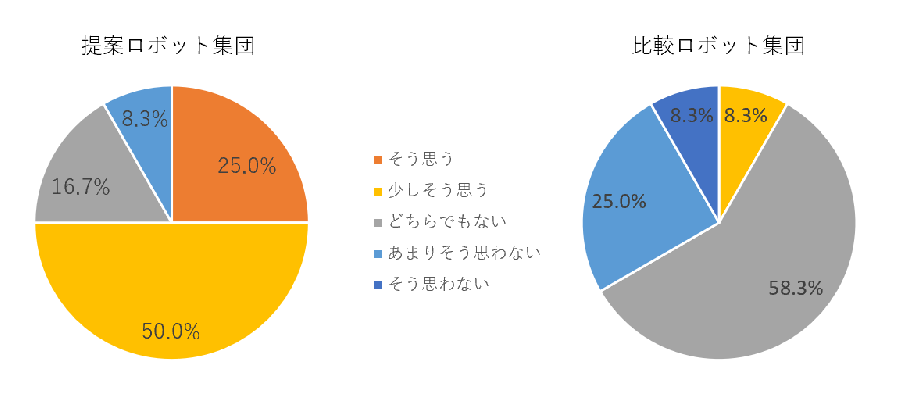
\includegraphics[width=15cm]{images/chapter4/Q1.eps}
  \caption{「ロボット集団との観戦を楽しむことができたか」のアンケート結果}
  \label{Q1}
 \end{center}
\end{figure}



\begin{figure}[!h]
 \begin{center}
\vspace{3cm}
  \centering
  \includegraphics[width=15cm]{images/chapter4/Q2.eps}
  \caption{「実際にロボット集団は観戦しているように感じたか」のアンケート結果}
  \label{Q2}
 \end{center}
\end{figure}



\newpage

\begin{figure}[!h]
 \begin{center}
\vspace{3cm}
  \centering
  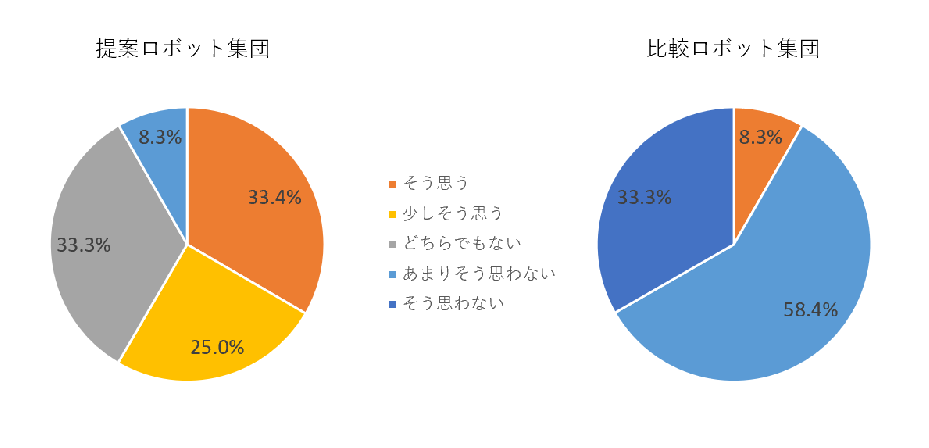
\includegraphics[width=15cm]{images/chapter4/Q3.eps}
  \caption{「ロボット集団との観戦で一体感を感じることができたか」のアンケート結果}
  \label{Q3}
 \end{center}
\end{figure}



\begin{figure}[!h]
 \begin{center}
\vspace{2cm}
  \centering
  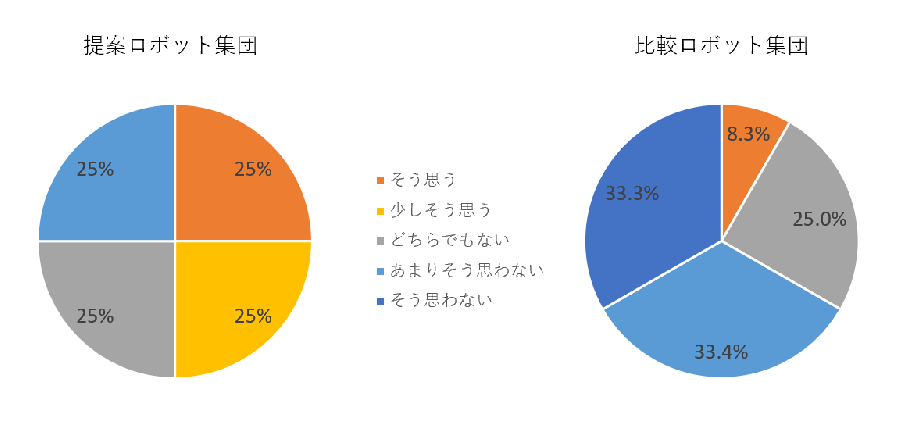
\includegraphics[width=15cm]{images/chapter4/Q4.eps}
  \caption{「ロボット集団との観戦で臨場感を感じることができたか」のアンケート結果}
  \label{Q4}
 \end{center}
\end{figure}

\newpage


\begin{figure}[!h]
 \begin{center}
\vspace{3cm}
  \centering
  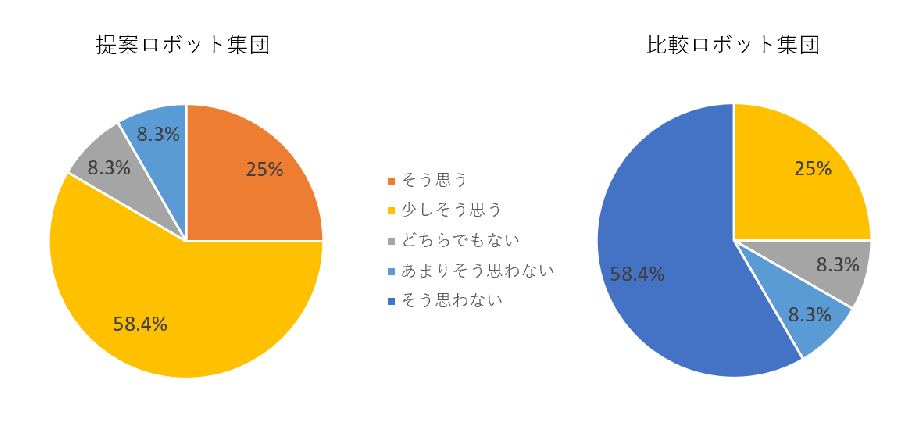
\includegraphics[width=15cm]{images/chapter4/Q5.eps}
  \caption{「ロボット集団の感情表出に感化されたか」のアンケート結果}
  \label{Q5}
 \end{center}
\end{figure}



\begin{figure}[!h]
 \begin{center}
\vspace{3cm}
  \centering
  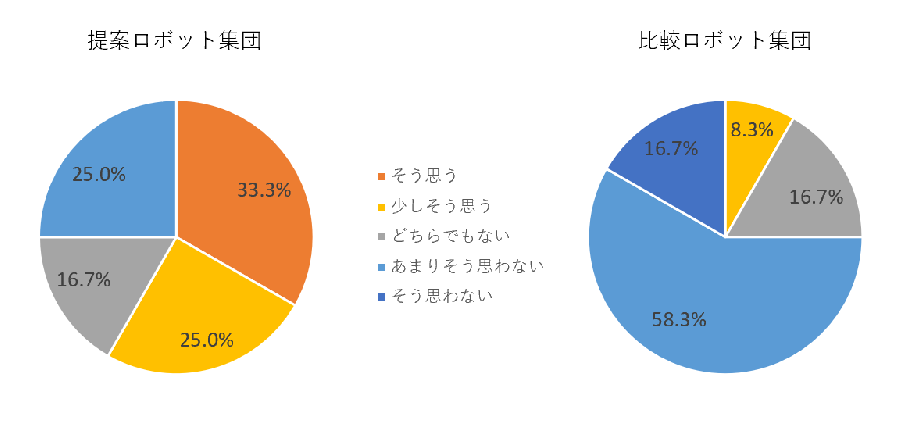
\includegraphics[width=15cm]{images/chapter4/Q6.eps}
  \caption{「ロボット集団に人間らしさを感じたか」のアンケート結果}
  \label{Q6}
 \end{center}
\end{figure}

\newpage



\begin{figure}[!h]
 \begin{center}
\vspace{3cm}
  \centering
  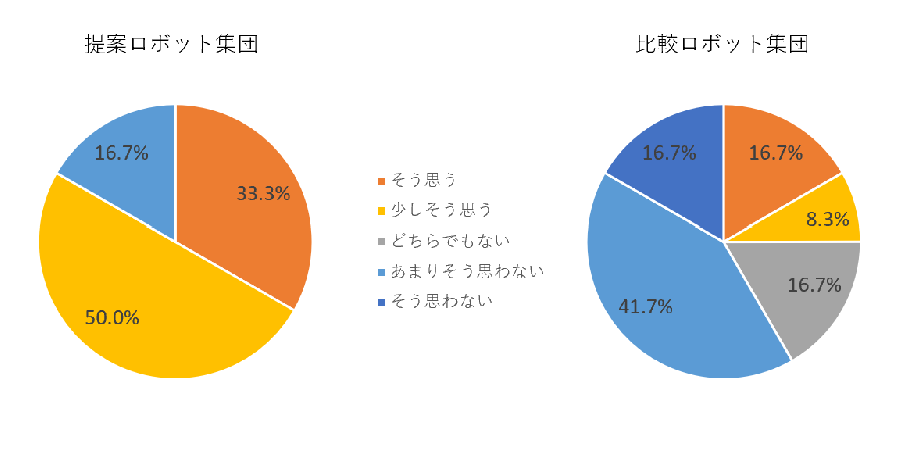
\includegraphics[width=15cm]{images/chapter4/Q7.eps}
  \caption{「ロボット集団に親しみを持てたか」のアンケート結果}
  \label{Q7}
 \end{center}
\end{figure}




\begin{figure}[!h]
 \begin{center}
\vspace{2cm}
  \centering
  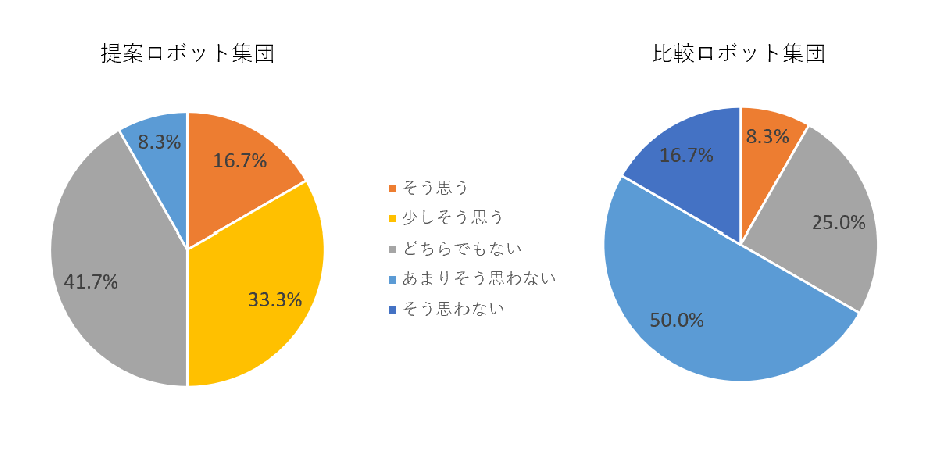
\includegraphics[width=15cm]{images/chapter4/Q8.eps}
  \caption{「またこのロボット集団と一緒に観戦したいか」のアンケート結果}
  \label{Q8}
 \end{center}
\end{figure}



\newpage

\vspace{1cm}
\begin{figure}[!h]
 \begin{center}
  \centering
  \includegraphics[width=15cm]{images/chapter4/Q9.eps}
  \caption{どちらのロボット集団の観戦が楽しかったか}
  \label{Q9}
 \end{center}
\end{figure}

\vspace{1cm}
\begin{figure}[!h]
 \begin{center}
  \centering
  \includegraphics[width=15cm]{images/chapter4/Q10.eps}
  \caption{どちらのロボット集団に一体感を感じたか}
  \label{Q10}
 \end{center}
\end{figure}

\newpage

\vspace{1cm}
\begin{figure}[!h]
 \begin{center}
  \centering
  \includegraphics[width=15cm]{images/chapter4/Q11.eps}
  \caption{どちらのロボット集団に臨場感を感じたか}
  \label{Q11}
 \end{center}
\end{figure}

\vspace{1cm}
\begin{figure}[!h]
 \begin{center}
  \centering
  \includegraphics[width=15cm]{images/chapter4/Q12.eps}
  \caption{どちらのロボット集団の感情表出に感化されたか}
  \label{Q12}
 \end{center}
\end{figure}

\newpage

\vspace{1cm}
\begin{figure}[!h]
 \begin{center}
  \centering
  \includegraphics[width=15cm]{images/chapter4/Q13.eps}
  \caption{どちらのロボット集団に人間らしさを感じたか}
  \label{Q13}
 \end{center}
\end{figure}

\vspace{1cm}
\begin{figure}[!h]
 \begin{center}
  \centering
  \includegraphics[width=15cm]{images/chapter4/Q14.eps}
  \caption{どちらのロボット集団に親しみを持てたか}
  \label{Q14}
 \end{center}
\end{figure}

\newpage

\vspace{1cm}
\begin{figure}[!h]
 \begin{center}
  \centering
  \includegraphics[width=15cm]{images/chapter4/Q15.eps}
  \caption{どちらのロボット集団とまた一緒に観戦したいか}
  \label{Q15}
 \end{center}
\end{figure}





\newpage

\section{考察}
\label{sec4.4}

図\ref{Q1}より,頻繁に感情を表出するロボット集団との観戦で,被験者は楽しさを感じていたことが分かる.これは,実空間での観戦を提案ロボット集団との観戦で再現できていたためだと考えられる.また,図\ref{Q2}~図\ref{Q5}より,被験者は提案ロボット集団との観戦で,本研究で示している臨場感の構成要素である,没入感や一体感,ロボット集団からの感情伝播に関する評価が高かったことが分かる.一方で,臨場感そのものについて問う質問では,半数の被験者がどちらでもない,あるいは低評価だと回答しており,十分な結果とは言えなかった.この結果から,没入感や一体感,感情伝播以外にも,スポーツ観戦において,臨場感を演出するために必要な要素があると考えられる.

両ロボットを比較する質問である図\ref{Q9}~図\ref{Q15}より,被験者の9割以上が,提案ロボット集団の方が,共に試合観戦を行うロボット集団に適していると感じていたことが分かる.この結果から,スポーツ観戦において臨場感を演出するためには,周囲の感情表出が必要不可欠であると考えられる.一方で,比較ロボット集団の方が適していると回答した被験者はほとんどいなかった.これは,本実験で設定したパラメータにより,提案ロボット集団と比較ロボット集団の感情表出のしやすさに差を付けすぎたことが原因であると考えられる.

また,自由記述で「ロボット集団が動作に合わせて歓声を挙げた方がいいと思った」「ロボット同士のハイタッチなどがあればより観戦していると感じることができると思った」などのロボットの感情表出に関する記述が多かった.一方で,「動作だけでも一体になっている感覚があった」という記述もあった.これらの記述から,観戦するロボットの動作による感情表出だけでも臨場感を演出することはできているが,感情表出の方法をより工夫することで,更なる臨場感の演出が期待できると考えられる.
















% !TEX root = MasterPaper.tex
\chapter{結論}
\thispagestyle{fancy}
\lhead{}
\chead{}
\rhead{}
\lfoot{} 
\cfoot{\thepage}
\rfoot{}

本研究では,スポーツ観戦における臨場感演出のためのロボット集団の振る舞いについて調査した.
先行研究では,人と顔表情で感性表現をするロボットとのコミュニケーションによって,ユーザに親しみやすい印象を与えていた.しかし,先行研究のシチュエーションでは,ロボット集団とのコミュニケーションは考えられていない.また,臨場感に関する先行研究,「興奮」や「面白さ」は臨場感を高めるための重要な要素であることが明らかになっていた.しかし,先行研究ではロボットとのインタラクションで臨場感を感じるかどうかは検証されていない.

そのため,本研究では,感情表出するロボット集団とスポーツ観戦を行うことで,ロボット集団から人への感情伝播が起こるかを検証した.また,ロボット集団との観戦によって起こる没入感や一体感,感情伝播によって臨場感を演出することは可能かを検証した.

第2章では,まず臨場感の定義についての先行研究,臨場感を感じる事象の分析についての先行研究を述べた.
次に,スポーツ観戦において臨場感を演出するための要素について述べた.
続いて,ロボットの進化についてと,ロボットへ感性を導入する意義について述べた.
最後に,ロボット集団と人間が円滑にインタラクションを行うためのロボット集団の設計について述べた.

第3章では,本研究で提案するロボット集団の内部モデル,本実験で用いた実験環境とロボット集団の動作について述べた.まず初めに,ロボット集団が実際に観戦を行っているように演出するため,勝利確率を読み取って感情生成を行うモデルについて述べた.次に,本実験で用いた環境について述べた.本実験では,ロボット集団との観戦で臨場感を演出するために,スポーツバーを模した空間を制作した.最後に,本実験で用いたロボットの動作について述べた.

第4章では,実ユーザによる評価実験について述べた.まず初めに,観戦する試合映像と,ロボット集団のパラメータについて述べた.次に,感情表出をするロボット集団との野球観戦でユーザが臨場感を感じるのかを検証した実験について述べた.被験者は提案ロボット集団と比較ロボット集団の両方と野球観戦を行い,その後アンケートを用いてそれぞれのロボット集団への印象評価と比較を行った.最後に,アンケートの結果を用いて提案ロボット集団の有効性について検討した.

本実験の結果から,提案ロボット集団との観戦で,ロボット集団からユーザに感情伝播が起こり,それによって起こる没入感や一体感によって,臨場感を感じることが分かった.
今後の課題としては,ロボット集団内でのロボット同士の感情伝播や,ロボットの表出感情の改良による更なる臨場感の演出が挙げられる.


\chapter*{謝辞}
\addcontentsline{toc}{chapter}{謝辞}

本研究を行うにあたり,日ごろから暖かいご指導を賜りました,徳丸正孝教授,Emmanuel Ayedoun助教に心より御礼申し上げます.また,さまざまな面でご支援いただいた,感性情報システム研究室の布施陽太郎氏,井上聡子氏,川合巧人氏,Wang Lingkai 氏,井下魁人氏,中田哲史氏,吉田朗大氏,
渡辺健吾氏,石川智稀氏,遠藤美咲氏,小池雄貴氏,小林陸門氏,酒部佑介氏,隅田汀央氏,田村優斗氏,中西優太氏,奈良樹氏, 
野本涼太氏に深く感謝致します.

%\UTF{9534}%

% !TEX root = MasterPaper.tex
\renewcommand{\bibname}{参考文献}
\addcontentsline{toc}{chapter}{参考文献}

\begin{thebibliography}{27} %{}内に参考文献の総数を書く

%序論

\bibitem{hamasuta}
% バーチャルハマスタ,``https:\slash\slash{}www.au.com\slash{}sports\slash{}baseball\slash{}articles\_virtual\_hamasta202103\slash{}'',
バーチャルハマスタ,``https://www.au.com/sports/baseball/articles\_virtual\_\\hamasta202103/'',
最終閲覧日:2022/2/1.

\bibitem{healsio}
ウォーターオーブン ヘルシオ:シャープ,``http://healsio.jp/'',最終閲覧日:2022/2/1.

\bibitem{go}
D.Silver,A.Huang,C.J.Maddison,A.Guez,L.Sifre,G.v.d.Driessche,J.Schrittwieser,I.Antonoglou,V.Panneershelvam,M.Lanctot,S.Dieleman,
D.Grewe,J.Nham,N.Kalchbrenner,I.Sutskever,T.Lillicrap,M.Leach,K.Kavukcuoglu,T.Graepel,D.Hassabis,
``Mastering the game of Go with deep neural networks and tree search'',Nature 529, pp.484-489, 2016.

\bibitem{toyota}
トヨタ-パーソナルロボット,``https://www.toyota.co.jp/jpn/tech/partner\_robot/'',最終閲覧日:2022/2/1.

\bibitem{aibo}
aibo,``http://aibo.sony.jp/'',最終閲覧日:2022/2/1.

\bibitem{deep}
松尾豊,``人工知能は人間を超えるか --ディープランニングの先にあるもの--'',KADOKAWA/中経出版,2015.

\bibitem{kao}
小林宏,原文雄,内田豪,大野宗久,``アクティブ・ヒューマン・インターフェース(AHI)のための顔ロボットの研究 
-顔ロボットの機構と6基本表情の表出-'',日本ロボット学会誌,vol.12,no.1,pp.155-163,1994.

\bibitem{syuwa}
三輪敬之,``手話ロボットハンド'',日本ロボット学会誌,vol.7,no.3,pp.113,1989.

\bibitem{higengo}
菅野重樹,渋谷恒司,``非言語コミュニケーションのための人間形ロボット'',日本ロボット学会誌,vol.15,no.7,pp.975-978,1997.

%2章

\bibitem{rinjyo1}
谷口高士,``臨場感の構成概念と評価について'',大阪学院大学,人文自然論叢,
第69-70号,2015.

\bibitem{lombard}
M.Lombard,T.Ditton,``At the heart of it all: The concept of presence'',Journal of Computer-Mediated Communication,3,online,1997.

\bibitem{ando}
安藤広志,``超臨場感に対する五感・認知'',原島博(監修)・映像情報メディア学会(編),超臨場感システム,オーム社,194-199,2010.

\bibitem{rinjyo2}
寺本渉,吉田和博,浅井暢子,日高聡太,行場次朗,鈴木陽一,``臨場感の素朴な理解'',
日本バーチャルリアリティ学会論文誌,Vol.105,No.1,2010.

\bibitem{rinjyo3}
橋本泰裕,中田大貴,``歓声量から観客を興奮させるプレーを評価する'',体力測定評価研究,2019.

\bibitem{ittai}
塹江清志,水野和夫,塹江光子,``「一体感」と「断絶感」'',名古屋工業大学紀要,50巻,p.185-190,1999-03-31.

\bibitem{denpa}
安藤和代,``ポジティブなクチコミにおいて非言語要素が誘発する感情伝播効果'',千葉商大論叢,51巻1号,pp.63-82,2013.

\bibitem{jyodo}
F.M.Gotz,S.Stiegert,T.Ebert,P.J.Rentfrow,D.Lewetz,`` What Drives Our Emotions When We Watch Sporting Events? An ESM Study on the Affective Experience of German Spectators During the 2018 FIFA World Cup''
,Collabra,Psychology,6(1),15,DOI,2020.

\bibitem{perso}
伊藤俊樹,長田純一,山口智治,藤田善弘,市川玲,江角彩,近藤安津美,近藤龍彰,
``パーソナルロボット「パペロ」に対する好意度尺度の作成'',日本デザイン学会研究発表大会概要集,日本デザイン学会,
第58回研究発表大会,一般社団法人,日本デザイン学会,2011.

\bibitem{gengo}
後藤みの理, 加納政芳, 加藤昇平, 國立勉, 伊藤英則, ``感性ロボットのための感情領域を用いた表情生成'', 
人工知能学会論文誌, 21巻1号G, 2006.

\bibitem{tekiou}
高岡勇紀, 尾関基行, 岡夏樹, ``人とロボットの相互適応過程を考慮したロボットの学習方法'', 
電子情報通信学会技術研究報告ヒューマンコミュニケーション基礎研究会, Vol114, 
No517, HCS2014-125, pp.75-80, 2015.

\bibitem{rabot}
らぼっと,``https://lovot.life/'',最終閲覧日:2022/1/7.

%3章

\bibitem{kyusute}
キューステ!, ``https://sports-station.jp/'', 最終閲覧日:2022/1/23.

\bibitem{unity}
Unity, ``https://unity.com/'', 最終閲覧日:2022/1/23.

\bibitem{bar}
Sports Bar 01,``https://assetstore.unity.com/packages/3d/environments/sport-bar-01-194104'',最終閲覧日:2022/1/23.

\bibitem{lilrobot}
Lil Robots with changeable expressions,``https://assetstore.unity.com/packages/\\3d/characters/robots/lil-robots-with-changeable-expressions-147408'',\\最終閲覧日:2022/1/23.

\bibitem{vive}
VIVE, ``https://www.vive.com/'', 最終閲覧日:2022/1/23.

%4章

\bibitem{patv}
パ・リーグTV,``https://tv.pacificleague.jp/ptv/pc/'',最終閲覧日:2022/1/29.




\end{thebibliography}
%
\pagestyle{empty}
%
\end{document}